\documentclass[12pt,english]{article}\usepackage[]{graphicx}\usepackage[usenames, dvipsnames]{xcolor}
% maxwidth is the original width if it is less than linewidth
% otherwise use linewidth (to make sure the graphics do not exceed the margin)
\makeatletter
\def\maxwidth{ %
  \ifdim\Gin@nat@width>\linewidth
    \linewidth
  \else
    \Gin@nat@width
  \fi
}
\makeatother

\definecolor{fgcolor}{rgb}{0.345, 0.345, 0.345}
\newcommand{\hlnum}[1]{\textcolor[rgb]{0.686,0.059,0.569}{#1}}%
\newcommand{\hlstr}[1]{\textcolor[rgb]{0.192,0.494,0.8}{#1}}%
\newcommand{\hlcom}[1]{\textcolor[rgb]{0.678,0.584,0.686}{\textit{#1}}}%
\newcommand{\hlopt}[1]{\textcolor[rgb]{0,0,0}{#1}}%
\newcommand{\hlstd}[1]{\textcolor[rgb]{0.345,0.345,0.345}{#1}}%
\newcommand{\hlkwa}[1]{\textcolor[rgb]{0.161,0.373,0.58}{\textbf{#1}}}%
\newcommand{\hlkwb}[1]{\textcolor[rgb]{0.69,0.353,0.396}{#1}}%
\newcommand{\hlkwc}[1]{\textcolor[rgb]{0.333,0.667,0.333}{#1}}%
\newcommand{\hlkwd}[1]{\textcolor[rgb]{0.737,0.353,0.396}{\textbf{#1}}}%
\let\hlipl\hlkwb

\usepackage{framed}
\makeatletter
\newenvironment{kframe}{%
 \def\at@end@of@kframe{}%
 \ifinner\ifhmode%
  \def\at@end@of@kframe{\end{minipage}}%
  \begin{minipage}{\columnwidth}%
 \fi\fi%
 \def\FrameCommand##1{\hskip\@totalleftmargin \hskip-\fboxsep
 \colorbox{shadecolor}{##1}\hskip-\fboxsep
     % There is no \\@totalrightmargin, so:
     \hskip-\linewidth \hskip-\@totalleftmargin \hskip\columnwidth}%
 \MakeFramed {\advance\hsize-\width
   \@totalleftmargin\z@ \linewidth\hsize
   \@setminipage}}%
 {\par\unskip\endMakeFramed%
 \at@end@of@kframe}
\makeatother

\definecolor{shadecolor}{rgb}{.97, .97, .97}
\definecolor{messagecolor}{rgb}{0, 0, 0}
\definecolor{warningcolor}{rgb}{1, 0, 1}
\definecolor{errorcolor}{rgb}{1, 0, 0}
\newenvironment{knitrout}{}{} % an empty environment to be redefined in TeX

\usepackage{alltt}
\usepackage[usenames, dvipsnames]{xcolor}
\usepackage[top=2cm, bottom=2cm, left=2.5cm, right=2.5cm]{geometry}
\usepackage[T1]{fontenc}
\usepackage{inputenc}
\usepackage{parskip}
\setlength{\parindent}{0pt}
\usepackage{amsmath}
\usepackage{caption}
\usepackage{url}
\usepackage[bookmarksnumbered]{hyperref}
\hypersetup{colorlinks, citecolor=RoyalBlue, linkcolor=RubineRed, urlcolor=MidnightBlue}
\hypersetup{pdfauthor={Constantin Manuel Bosancianu},
pdftitle={Measures of fit in MLM},
pdfsubject={Measures of fit for multilevel models},
pdfkeywords={multilevel, fit statistics, likelihood, AIC, BIC}}
\usepackage{babel}
\usepackage{graphicx}
\usepackage{CormorantGaramond}
\usepackage{dcolumn}
\usepackage{setspace}
\onehalfspacing
\usepackage{titlesec}
\titleformat{\section}{\large\bfseries}{\thesection}{0.4em}{}
\titleformat{\subsection}{\normalfont\bfseries}{\thesubsection}{0.2em}{}
\usepackage{booktabs}
\setlength{\heavyrulewidth}{0.2em}
\usepackage{apacite}
\bibliographystyle{apacite}
\makeatletter
\renewcommand{\maketitle}{
  \begin{flushleft}
    {\huge\@title}\\
    \vspace{10pt}
    {\large\@author}\\
    {\@date}
    \vspace{40pt}
  \end{flushleft}
}
\makeatother
\usepackage{authblk}
\title{\textsc{MLM measures of fit}}
\author{\textbf{Constantin Manuel Bosancianu}\footnote{You can reach me at \href{mailto:bosancianu@icloud.com}{bosancianu@icloud.com}. If you spot any mistakes I'd be grateful if you sent me an email pointing it out; I'll update the document and credit the help offered. One example was a small mistake concerning a subscript in equation \ref{eq:eq-5}, which Daniele Mantegazzi spotted in 2015 (thanks!).}}
\affil{WZB Berlin Social Science Center \\ \textit{Institutions and Political Inequality}}
\date{July 3, 2019}
\IfFileExists{upquote.sty}{\usepackage{upquote}}{}
\begin{document}
\maketitle

This will be a longer tutorial, focusing on measures of model fit commonly used in multilevel modeling, as well as on how to compare between models. Due to the estimation technique most commonly used (Maximum Likelihood), the measures of fit are reliant on the likelihood of the model, making interpretation slightly more difficult than in the case of a $R^2$ from OLS regression. In the following sections I will go through five of the most commonly used measures, after which I will focus on how we engage in model comparisons in the case of multilevel models.




\section{logLikelihood}
The first measure, produced directly by the estimation procedure, is the logarithm of the likelihood of the model. In very simple terms, glossing over some of the more technical details, the likelihood is the product of the densities evaluated at the observations.\footnote{This very simple definition belongs to Isabel Canette, senior statistician at StataCorp LP.} Drawing on high school math, the logarithm of a product is the sum of logarithms of the individual terms that constitute the product.

\begin{equation}
\label{eq:eq-1}
log(abc)=log(a)+log(b)+log(c)
\end{equation}






\begin{figure}[!ht]
\centering
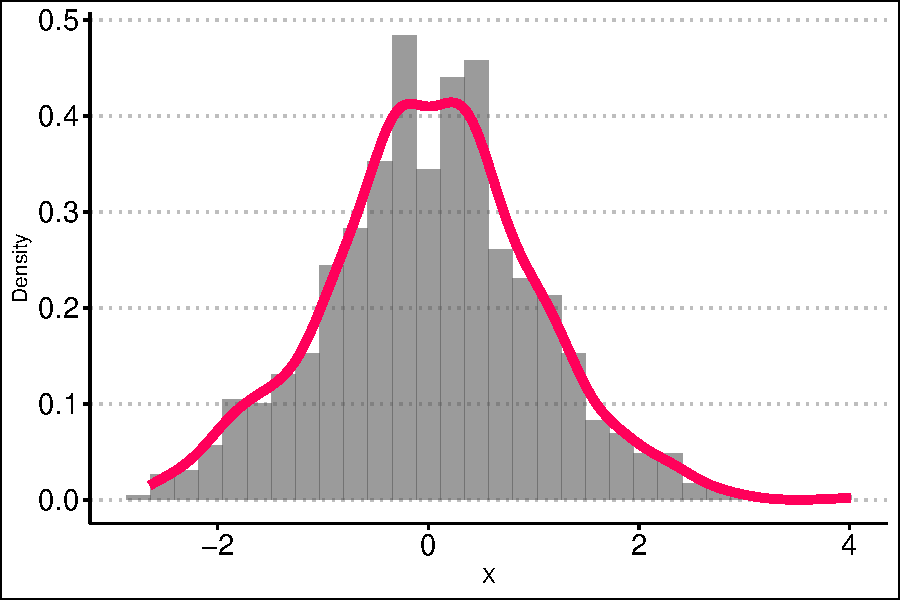
\includegraphics[width=0.6\linewidth]{../../05-graphs/Supplem-01}
\caption[Normal density plot]{Normal density plot}
\label{fig:fig-1}
\end{figure}

With a large sample size, the densities will usually all be much smaller than 1 (see Figure \ref{fig:fig-1} on page \pageref{fig:fig-1}), making the individual logarithms each smaller than 0 (the natural logarithm of any quantity smaller than 1 will be negative). The sum of these negative quantities will itself be negative, producing the usual numbers reported in multilevel regression tables for the logarithm of the likelihood. Most often times, then, the \textit{logLikelihood} will be a very small negative number, e.g. -12075.45.\footnote{At the end of this tutorial I'll indicate a situation where this no longer applies.} The \textit{logLikelihood} is a measure of fit that indicates how well our model fits the data: smaller values (farther away from 0) indicate models which fit the data worse.



\section{Deviance}
The \textit{deviance} is computed as $-2 \times logLikelihood$, which makes it an indicator of model misfit: higher values (farther away from 0) indicate a worse fitting model. More about the deviance in a following section; for now, this simple formula will suffice.


\section{AIC and BIC}
The \textit{Akaike Information Criterion} (AIC) is a simple extension of the logLikelihood.

\begin{equation}
\label{eq:eq-2}
AIC=-2 \times logLikelihood + 2 \times k
\end{equation}

In equation \ref{eq:eq-2}, $k$ represents the number of parameters estimated by our model. Unlike the deviance, the AIC includes a penalty for the number of parameters estimated in the model. When comparing two models this means that, \textit{ceteris paribus}, the model with fewer parameters will receive a lower AIC score, suggesting a slightly better fit to the data.

The \textit{Bayesian Information Criterion} (BIC), on the other hand, introduces a penalization both for number of parameters estimated and for the sample size.

\begin{equation}
\label{eq:eq-3}
BIC=-2 \times logLikelihood + k \times ln(N)
\end{equation}

In equation \ref{eq:eq-3}, $k$ continues to represent the number of parameters estimated by the model, while $N$ is the sample size.\footnote{\citeA{singer_applied_2003} recommend using the level 1 sample size.} We can see from the formula that larger sample sizes result in larger penalties and, therefore, in poorer fitting models. The ability of the BIC to incorporate both penalties has sometimes led to its use in comparing models estimated on different samples. Although this can sometimes be acceptable, in truth we know little about the behavior of the BIC under different model specifications and sample configurations. Because of this, my advice here is to avoid using this measure in these instances.




\section{R\textsuperscript{2}}

A final measure, proposed by \citeA{snijders_multilevel_1999} under the name $R^2$, assesses the extent to which a more complex model reduces the prediction error (interpreted here as the magnitude of the residuals), compared to a less complex model \cite[p.~35]{luke_multilevel_2004}. Considering two models, $M_1$ and $M_2$, where $M_2$ includes all of the parameters in $M_1$ plus a few more, and that $var(u_{0j})=\tau_0^2$ and $var(r_{ij})=\sigma^2$, then we can write the formula\footnote{In this tutorial I presented formulas as they are reported by \citeauthor[pp.~35--36]{luke_multilevel_2004}, as these are more accessible to a new audience than the ones offered by \citeA{snijders_multilevel_1999}.} for $R^2$ at the level 1 as

\begin{equation}
\label{eq:eq-4}
R_1^2=1 - \frac{(\sigma^2 + \tau_0^2)_{model2}}{(\sigma^2 + \tau_0^2)_{model1}}
\end{equation}

From equation \ref{eq:eq-4} we can see that the better $M_2$ manages to explain the variance in the residuals, the lower is the value of the fraction from the equation. At the extreme, when $M_2$ perfectly explains the residuals, $R_1^2=1-0=1$. A similar formula gives us the $R^2$ at the level 2:

\begin{equation}
\label{eq:eq-5}
R_2^2=1 - \frac{(\frac{\sigma^2}{n}+\tau_0^2)_{model 2}}{(\frac{\sigma^2}{n}+\tau_0^2)_{model 1}}
\end{equation}

The $n$ in equation \ref{eq:eq-5} designates the average number of level 1 units that are nested in level 2 units. The major benefit of the $R^2$ is that it is able to offer much more precise information than other indicators, as it captures changes at both levels of the hierarchy. On the other hand, in some instances adding a predictor might result, paradoxically, in a \textit{larger} variance of residuals, and therefore in a \textit{negative} $R^2$.




\section{Usage of the indicators}
As you get started with using these you might find useful a few rough guidelines regarding the use of these indicators in practical applications. To begin with, except for the BIC, the indicators should only be used to compare two models which have been estimated on the same sample. Without such a restriction the researcher has no way of knowing whether the reduction in logLikelihood or AIC is due to the addition of a predictor in the model, or due to a different sample on which the model is tested. Theoretically speaking, the BIC could be used for comparing models estimated on different samples, as its formula includes a correction for sample size. In practice, though, this is rarely done, for the reasons outlined in the section which deals with this indicator.

A second guideline refers to the type of models which can be compared using these indicators. A conservative practice is to use the deviance and the AIC only for \textit{nested} models. By \textit{nested} models, I mean a configuration of two models whereby one includes all of the parameters of the other one, as well as a few extra ones. For example, if $M_1: Y=\beta_0+\beta_1X_1+e$ and $M_2: Y=\beta_0+\beta_1X_1+\beta_2X_2+e$, then $M_1$ is nested in $M_2$.

In truth, this is one of the more contentious issues in multilevel modeling, about which disagreement still persists. \citeA[p.~50]{hox_multilevel_2010}, \citeA[p.~35]{luke_multilevel_2004} and \citeA[p.~88]{burnham_model_2002} suggest that AIC can be used for non-nested models, while \citeA[p.~252]{hamaker_model_2011} endorse this view, heavily citing Burnham and Anderson for support. \citeA[p.~259]{pinheiro_mixed_2000} also take the view that AIC and BIC can be used for non-nested models. On the other hand, \citeA{ripley_selecting_2004} flatly states that AIC comparisons are only useful for nested models, a view which he expresses outside of his writings as well.\footnote{See the discussion at \url{http://r.789695.n4.nabble.com/Nested-AIC-td794191.html}, where Thomas Lumley seems to also endorse the view that AIC-based comparisons for non-nested models are somewhat risky. Somewhere else, Brian Ripley takes a more blunt approach toward the statements made by Burnham and Anderson in their book: \url{https://stat.ethz.ch/pipermail/r-help/2003-June/035526.html}.} \citeA[p.~122]{singer_applied_2003} suggest that one can use AIC and BIC to compare non-nested models, but urge researchers to only use them when more traditional methods of model comparison don't work. Furthermore, they advise caution when using them. At the same time, in a handout/presentation from 2003, the same authors only say that one can ``supposedly'' use these information criteria to engage in such comparisons.\footnote{See \url{http://gseacademic.harvard.edu/alda/Handouts/ALDA\%20Chapter\%204.pdf}.} It does seem that the weight of the evidence tends to favor the ``yes, we can!'' camp. I would advise some restraint, though, when engaging in such AIC-based comparisons of non-nested models: (1) don't compare models run with different R functions, as they might produce likelihoods that aren't comparable; (2) don't compare models in which one uses a transformation of the outcome, while the other  one doesn't.\footnote{In his response to the discussion at \url{http://r.789695.n4.nabble.com/Nested-AIC-td794191.html} Thomas Lumley outlines a few more situations where AIC should not be used for non-nested models.}

Finally, a measure of caution should be used with respect to the AIC/BIC and FIML or REML estimation. When using FIML estimation, models that differ either in fixed effects or random effects can be compared with the AIC or BIC. When relying on REML estimation, though, only models that differ in random effects can be compared \cite[p.~51]{hox_multilevel_2010}.





\section{Trivia: can the logLikelihood be positive as well?}




\begin{figure}[!ht]
\centering
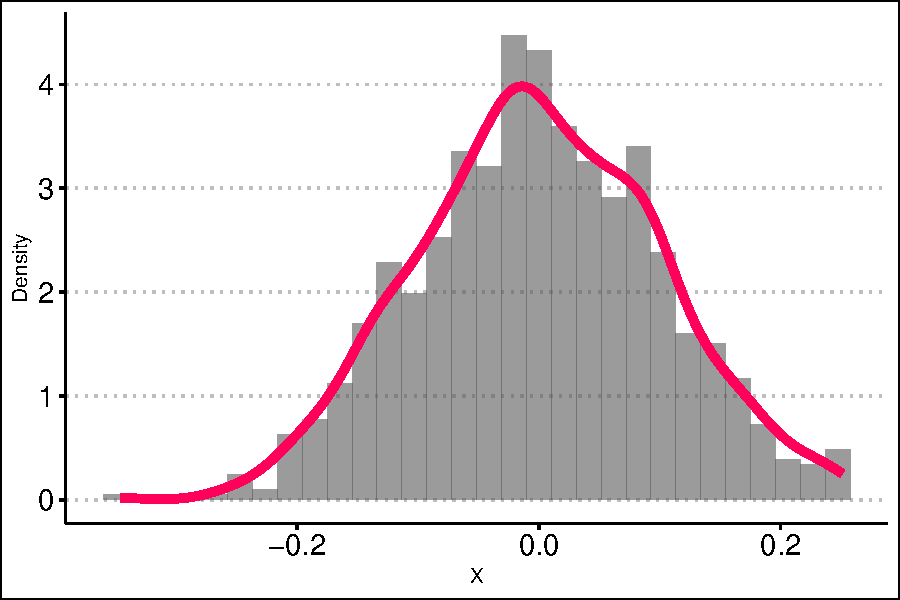
\includegraphics[width=0.6\linewidth]{../../05-graphs/Supplem-02}
\caption[Normal density plot]{Normal density plot with very low variance}
\label{fig:fig-2}
\end{figure}

In a few instances, yes, it can. If you remember from the introductory part of this document, the likelihood is computed as the product of the densities evaluated at the observations. When taking the logarithm of this quantity, we obtain a sum of logarithms of densities. As long as the distribution looks similar to the one presented in Figure \ref{fig:fig-1}, with a normal degree of dispersion, the \textit{logLikelihood} should be negative on account of each element in that sum being negative. Consider what would happen, though, if the distribution would have a very low variance, as the one presented in Figure \ref{fig:fig-2}.

In this instance, a considerable number of elements have a density above 1, which means that their logarithm will have a positive value. If our distribution has a lot of these elements, then it's possible that the logLikelihood will be positive.

\bibliography{../../references}

\end{document}
